% From https://github.com/UWIT-IAM/UWThesis

\documentclass [11pt, proquest] {uwthesis}[2015/03/03]


% fix for pandoc 1.14
\providecommand{\tightlist}{%
  \setlength{\itemsep}{0pt}\setlength{\parskip}{0pt}}

\newtheorem{theorem}{Jibberish}

%% \bibliography{references}

\hyphenation{mar-gin-al-ia}

%
% ----- apply watermark to every page
% ----- change 'stamp' to 'nostamp'
%------ to omit watermark
%
\usepackage[nostamp]{draftwatermark}
% % Use the following to make modification
\SetWatermarkText{DRAFT}
\SetWatermarkLightness{0.95}

%% for the per mil symbol
\usepackage[nointegrals]{wasysym}

%% for copyright symbol
\usepackage{textcomp}

%% to allow to rotate pages to landscape
\usepackage{lscape}
%% to adjust table column width
\usepackage{tabularx}

% suppress bottom page numbers on first page of each chapter
% because they overlap with text
\usepackage{etoolbox}
\patchcmd{\chapter}{plain}{empty}{}{}

%% for more attractive tables
\usepackage{booktabs}
\usepackage{longtable}


\usepackage{graphicx}


% Double spacing, if you want it.
% \def\dsp{\def\baselinestretch{2.0}\large\normalsize}
% \dsp

% If the Grad. Division insists that the first paragraph of a section
% be indented (like the others), then include this line:
% \usepackage{indentfirst}

%%%%%%%%%%%%%%%%%%
% If you want to use "sections" to partition your thesis
% un-comment the following:
%
% \counterwithout{section}{chapter}
% \setsecnumdepth{subsubsection}
% \def\sectionmark#1{\markboth{#1}{#1}}
% \def\subsectionmark#1{\markboth{#1}{#1}}
% \renewcommand{\thesection}{\arabic{section}}
% \renewcommand{\thesubsection}{\thesection.\arabic{subsection}}
% \makeatletter
% \let\l@subsection\l@section
% \let\l@section\l@chapter
% \makeatother
%
% \renewcommand{\thetable}{\arabic{table}}
% \renewcommand{\thefigure}{\arabic{figure}}
%
%%%%%%%%%%%%%%%%%%


%% Stuff from https://github.com/suchow/Dissertate

% The following line would print the thesis in a postscript font

% \usepackage{natbib}
% \def\bibpreamble{\protect\addcontentsline{toc}{chapter}{Bibliography}}

\setcounter{tocdepth}{1} % Print the chapter and sections to the toc
% controls depth of table of contents (toc): 0 = chapter, 1 = section, 2 = subsection

\usepackage{biblatex}

\prelimpages

%% from thesisdown
% To pass between YAML and LaTeX the dollar signs are added by CII
\Title{Diabetes and Public Housing}
\Author{Marc Macarulay}
\Year{2020}
\Program{Health Services}
\Chair{}{}{Health Services}
\Signature{}
\Signature{}
\Signature{}

% commands and environments needed by pandoc snippets
% extracted from the output of `pandoc -s`
%% Make R markdown code chunks work
\usepackage{array}
\usepackage{amssymb,amsmath}
\usepackage{ifxetex,ifluatex}
\ifxetex
  \usepackage{fontspec,xltxtra,xunicode}
  \defaultfontfeatures{Mapping=tex-text,Scale=MatchLowercase}
\else
  \ifluatex
    \usepackage{fontspec}
    \defaultfontfeatures{Mapping=tex-text,Scale=MatchLowercase}
  \else
    \usepackage[utf8]{inputenc}
  \fi
\fi
\usepackage{color}
\usepackage{fancyvrb}
\DefineShortVerb[commandchars=\\\{\}]{\|}
\DefineVerbatimEnvironment{Highlighting}{Verbatim}{commandchars=\\\{\}}
% Add ',fontsize=\small' for more characters per line
\newenvironment{Shaded}{}{}
\newcommand{\KeywordTok}[1]{\textcolor[rgb]{0.00,0.44,0.13}{\textbf{{#1}}}}
\newcommand{\DataTypeTok}[1]{\textcolor[rgb]{0.56,0.13,0.00}{{#1}}}
\newcommand{\DecValTok}[1]{\textcolor[rgb]{0.25,0.63,0.44}{{#1}}}
\newcommand{\BaseNTok}[1]{\textcolor[rgb]{0.25,0.63,0.44}{{#1}}}
\newcommand{\FloatTok}[1]{\textcolor[rgb]{0.25,0.63,0.44}{{#1}}}
\newcommand{\CharTok}[1]{\textcolor[rgb]{0.25,0.44,0.63}{{#1}}}
\newcommand{\StringTok}[1]{\textcolor[rgb]{0.25,0.44,0.63}{{#1}}}
\newcommand{\CommentTok}[1]{\textcolor[rgb]{0.38,0.63,0.69}{\textit{{#1}}}}
\newcommand{\OtherTok}[1]{\textcolor[rgb]{0.00,0.44,0.13}{{#1}}}
\newcommand{\AlertTok}[1]{\textcolor[rgb]{1.00,0.00,0.00}{\textbf{{#1}}}}
\newcommand{\FunctionTok}[1]{\textcolor[rgb]{0.02,0.16,0.49}{{#1}}}
\newcommand{\RegionMarkerTok}[1]{{#1}}
\newcommand{\ErrorTok}[1]{\textcolor[rgb]{1.00,0.00,0.00}{\textbf{{#1}}}}
\newcommand{\NormalTok}[1]{{#1}}
\newcommand{\OperatorTok}[1]{\textcolor[rgb]{0.00,0.44,0.13}{\textbf{{#1}}}}
\newcommand{\BuiltInTok}[1]{\textcolor[rgb]{0.00,0.44,0.13}{\textbf{{#1}}}}
\newcommand{\ControlFlowTok}[1]{\textcolor[rgb]{0.00,0.44,0.13}{\textbf{{#1}}}}


\ifxetex
  \usepackage[setpagesize=false, % page size defined by xetex
              unicode=false, % unicode breaks when used with xetex
              xetex,
              colorlinks=true,
              linkcolor=blue]{hyperref}
\else
  \usepackage[unicode=true,
              colorlinks=true,
              linkcolor=blue]{hyperref}
\fi
\hypersetup{breaklinks=true, pdfborder={0 0 0}}
\setlength{\parindent}{0pt}
\setlength{\parskip}{6pt plus 2pt minus 1pt}
\setlength{\emergencystretch}{3em}  % prevent overfull lines
\setcounter{secnumdepth}{2} %% controls section numbering, e.g. 1 or 1.2, or 1.2.3

\begin{document}
\titlepage
  \pagebreak


\copyrightpage

\setcounter{page}{-1}
\abstract{``Here is my abstract''}

\tableofcontents
\listoffigures
\listoftables



\textpages


\chapter{Background and Significance}\label{rmd-basics}

\section{Problem Defintion}\label{problem-defintion}

Diabetes is a chronic disease that is characterized by an inability of
the body to maintain a healthy blood glucose level, this can cause a
variety of symptoms that affect multiple systems in the body and can
lead to potentially life-threatening complications.The key regulator
hormone of glucose is insulin and it is produced in the pancreas. The
absence or malfunction of insulin leads to elevated blood glucose levels
called hyperglycemia. When insulin hormone is missing or ineffective the
disease is called Diabetes Mellitus, this condition has multiple types.

\subsection{Diabetes Variants}\label{diabetes-variants}

The most common diabetes variants include type I diabetes mellitus, type
II diabetes mellitus, and gestational diabetes. Type I diabetes is
usually caused by genetic factors triggering an autoimmune reaction that
results in the destruction of insulin producing cells in the pancreas.
Also known as Juvenile Diabetes, the type I classification is typically
diagnosed relatively early in life during childhood or early adulthood.
Whereas, Type II diabetes develops when the body can still produce
insulin however the amount is insuffient or when the body becomes
resistant to the effects of insulin. Type II diabetes is largely
attributed to lifestyle factors including obesity and physical activity
levels.

This is a test to see if I can reference(Keene, Guo, \& Murillo, 2018)

Here is a brief introduction into using \emph{R Markdown}.
\emph{Markdown} is a simple formatting syntax for authoring HTML, PDF,
and MS Word documents. \emph{R Markdown} provides the flexibility of
\emph{Markdown} with the implementation of \textbf{R} input and output.
For more details on using \emph{R Markdown} see
\url{http://rmarkdown.rstudio.com}.

Be careful with your spacing in \emph{Markdown} documents. While
whitespace largely is ignored, it does at times give \emph{Markdown}
signals as to how to proceed. As a habit, try to keep everything left
aligned whenever possible, especially as you type a new paragraph. In
other words, there is no need to indent basic text in the Rmd document
(in fact, it might cause your text to do funny things if you do).

\section{Lists}\label{lists}

It's easy to create a list. It can be unordered like
\begin{itemize}
\tightlist
\item
  Item 1
\item
  Item 2
\end{itemize}
or it can be ordered like
\begin{enumerate}
\def\labelenumi{\arabic{enumi}.}
\tightlist
\item
  Item 1
\item
  Item 2
\end{enumerate}
Notice that I intentionally mislabeled Item 2 as number 4.
\emph{Markdown} automatically figures this out! You can put any numbers
in the list and it will create the list. Check it out below.

To create a sublist, just indent the values a bit (at least four spaces
or a tab). (Here's one case where indentation is key!)
\begin{enumerate}
\def\labelenumi{\arabic{enumi}.}
\tightlist
\item
  Item 1
\item
  Item 2
\item
  Item 3
  \begin{itemize}
  \tightlist
  \item
    Item 3a
  \item
    Item 3b
  \end{itemize}
\end{enumerate}
\section{Line breaks}\label{line-breaks}

Make sure to add white space between lines if you'd like to start a new
paragraph. Look at what happens below in the outputted document if you
don't:

Here is the first sentence. Here is another sentence. Here is the last
sentence to end the paragraph. This should be a new paragraph.

\emph{Now for the correct way:}

Here is the first sentence. Here is another sentence. Here is the last
sentence to end the paragraph.

This should be a new paragraph.

\hypertarget{r-chunks}{\section{R chunks}\label{r-chunks}}

When you click the \textbf{Knit} button above a document will be
generated that includes both content as well as the output of any
embedded \textbf{R} code chunks within the document. You can embed an
\textbf{R} code chunk like this (\texttt{cars} is a built-in \textbf{R}
dataset):
\begin{Shaded}
\begin{Highlighting}[]
\KeywordTok{summary}\NormalTok{(cars)}
\end{Highlighting}
\end{Shaded}
\begin{verbatim}
     speed           dist       
 Min.   : 4.0   Min.   :  2.00  
 1st Qu.:12.0   1st Qu.: 26.00  
 Median :15.0   Median : 36.00  
 Mean   :15.4   Mean   : 42.98  
 3rd Qu.:19.0   3rd Qu.: 56.00  
 Max.   :25.0   Max.   :120.00  
\end{verbatim}
\section{Inline code}\label{inline-code}

If you'd like to put the results of your analysis directly into your
discussion, add inline code like this:
\begin{quote}
The \texttt{cos} of \(2 \pi\) is 1.
\end{quote}
Another example would be the direct calculation of the standard
deviation:
\begin{quote}
The standard deviation of \texttt{speed} in \texttt{cars} is 5.2876444.
\end{quote}
One last neat feature is the use of the \texttt{ifelse} conditional
statement which can be used to output text depending on the result of an
\textbf{R} calculation:
\begin{quote}
The standard deviation is less than 6.
\end{quote}
Note the use of \texttt{\textgreater{}} here, which signifies a
quotation environment that will be indented.

As you see with \texttt{\$2\ \textbackslash{}pi\$} above, mathematics
can be added by surrounding the mathematical text with dollar signs.
More examples of this are in {[}Mathematics and Science{]} if you
uncomment the code in {[}Math{]}.

\section{Including plots}\label{including-plots}

You can also embed plots. For example, here is a way to use the base
\textbf{R} graphics package to produce a plot using the built-in
\texttt{pressure} dataset:

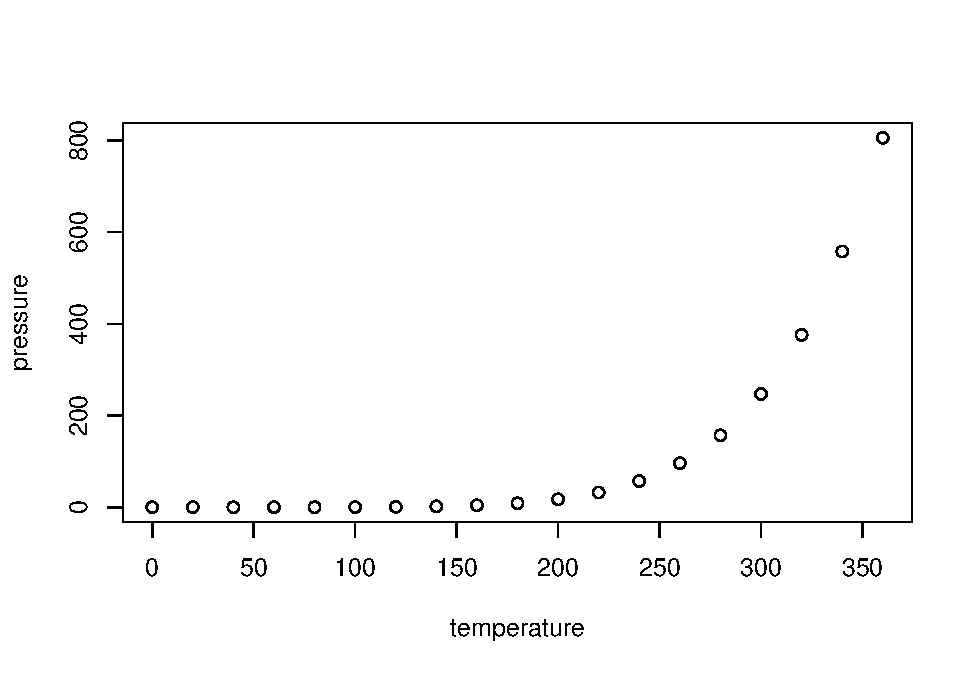
\includegraphics{Marc-Macarulay_files/figure-latex/pressure-1.pdf}

Note that the \texttt{echo=FALSE} parameter was added to the code chunk
to prevent printing of the \textbf{R} code that generated the plot.
There are plenty of other ways to add chunk options. More information is
available at \url{http://yihui.name/knitr/options/}.

Another useful chunk option is the setting of \texttt{cache=TRUE} as you
see here. If document rendering becomes time consuming due to long
computations or plots that are expensive to generate you can use knitr
caching to improve performance. Later in this file, you'll see a way to
reference plots created in \textbf{R} or external figures.

\hypertarget{loading-and-exploring-data}{\section{Loading and exploring
data}\label{loading-and-exploring-data}}

Included in this template is a file called \texttt{flights.csv}. This
file includes a subset of the larger dataset of information about all
flights that departed from Seattle and Portland in 2014. More
information about this dataset and its \textbf{R} package is available
at \url{http://github.com/ismayc/pnwflights14}. This subset includes
only Portland flights and only rows that were complete with no missing
values. Merges were also done with the \texttt{airports} and
\texttt{airlines} data sets in the \texttt{pnwflights14} package to get
more descriptive airport and airline names.

We can load in this data set using the following command:
\begin{Shaded}
\begin{Highlighting}[]
\NormalTok{flights <-}\StringTok{ }\KeywordTok{read.csv}\NormalTok{(}\StringTok{"data/flights.csv"}\NormalTok{)}
\end{Highlighting}
\end{Shaded}
The data is now stored in the data frame called \texttt{flights} in
\textbf{R}. To get a better feel for the variables included in this
dataset we can use a variety of functions. Here we can see the
dimensions (rows by columns) and also the names of the columns.
\begin{Shaded}
\begin{Highlighting}[]
\KeywordTok{dim}\NormalTok{(flights)}
\end{Highlighting}
\end{Shaded}
\begin{verbatim}
[1] 52808    16
\end{verbatim}
\begin{Shaded}
\begin{Highlighting}[]
\KeywordTok{names}\NormalTok{(flights)}
\end{Highlighting}
\end{Shaded}
\begin{verbatim}
 [1] "month"        "day"          "dep_time"     "dep_delay"    "arr_time"    
 [6] "arr_delay"    "carrier"      "tailnum"      "flight"       "dest"        
[11] "air_time"     "distance"     "hour"         "minute"       "carrier_name"
[16] "dest_name"   
\end{verbatim}
Another good idea is to take a look at the dataset in table form. With
this dataset having more than 50,000 rows, we won't explicitly show the
results of the command here. I recommend you enter the command into the
Console \textbf{\emph{after}} you have run the \textbf{R} chunks above
to load the data into \textbf{R}.
\begin{Shaded}
\begin{Highlighting}[]
\KeywordTok{View}\NormalTok{(flights)}
\end{Highlighting}
\end{Shaded}
While not required, it is highly recommended you use the \texttt{dplyr}
package to manipulate and summarize your data set as needed. It uses a
syntax that is easy to understand using chaining operations. Below I've
created a few examples of using \texttt{dplyr} to get information about
the Portland flights in 2014. You will also see the use of the
\texttt{ggplot2} package, which produces beautiful, high-quality
academic visuals.

We begin by checking to ensure that needed packages are installed and
then we load them into our current working environment:
\begin{Shaded}
\begin{Highlighting}[]
\CommentTok{# List of packages required for this analysis}
\NormalTok{pkg <-}\StringTok{ }\KeywordTok{c}\NormalTok{(}\StringTok{"dplyr"}\NormalTok{, }\StringTok{"ggplot2"}\NormalTok{, }\StringTok{"knitr"}\NormalTok{, }\StringTok{"bookdown"}\NormalTok{, }\StringTok{"devtools"}\NormalTok{)}
\CommentTok{# Check if packages are not installed and assign the}
\CommentTok{# names of the packages not installed to the variable new.pkg}
\NormalTok{new.pkg <-}\StringTok{ }\NormalTok{pkg[}\OperatorTok{!}\NormalTok{(pkg }\OperatorTok\StringTok{ }\KeywordTok{installed.packages}\NormalTok{())]}
\CommentTok{# If there are any packages in the list that aren't installed,}
\CommentTok{# install them}
\ControlFlowTok{if}\NormalTok{ (}\KeywordTok{length}\NormalTok{(new.pkg))}
  \KeywordTok{install.packages}\NormalTok{(new.pkg, }\DataTypeTok{repos =} \StringTok{"http://cran.rstudio.com"}\NormalTok{)}
\CommentTok{# Load packages (huskydown will load all of the packages as well)}
\KeywordTok{library}\NormalTok{(huskydown)}
\end{Highlighting}
\end{Shaded}
\clearpage

The example we show here does the following:
\begin{itemize}
\item
  Selects only the \texttt{carrier\_name} and \texttt{arr\_delay} from
  the \texttt{flights} dataset and then assigns this subset to a new
  variable called \texttt{flights2}.
\item
  Using \texttt{flights2}, we determine the largest arrival delay for
  each of the carriers.
\end{itemize}
\begin{Shaded}
\begin{Highlighting}[]
\KeywordTok{library}\NormalTok{(dplyr)}
\end{Highlighting}
\end{Shaded}
\begin{verbatim}

Attaching package: 'dplyr'
\end{verbatim}
\begin{verbatim}
The following objects are masked from 'package:stats':

    filter, lag
\end{verbatim}
\begin{verbatim}
The following objects are masked from 'package:base':

    intersect, setdiff, setequal, union
\end{verbatim}
\begin{Shaded}
\begin{Highlighting}[]
\NormalTok{flights2 <-}\StringTok{ }\NormalTok{flights }\OperatorTok
\StringTok{  }\KeywordTok{select}\NormalTok{(carrier_name, arr_delay)}
\NormalTok{max_delays <-}\StringTok{ }\NormalTok{flights2 }\OperatorTok
\StringTok{  }\KeywordTok{group_by}\NormalTok{(carrier_name) }\OperatorTok
\StringTok{  }\KeywordTok{summarize}\NormalTok{(}\DataTypeTok{max_arr_delay =} \KeywordTok{max}\NormalTok{(arr_delay, }\DataTypeTok{na.rm =} \OtherTok{TRUE}\NormalTok{))}
\end{Highlighting}
\end{Shaded}
A useful function in the \texttt{knitr} package for making nice tables
in \emph{R Markdown} is called \texttt{kable}. It is much easier to use
than manually entering values into a table by copying and pasting values
into Excel or LaTeX. This again goes to show how nice reproducible
documents can be! (Note the use of \texttt{results="asis"}, which will
produce the table instead of the code to create the table.) The
\texttt{caption.short} argument is used to include a shorter title to
appear in the List of Tables.
\begin{Shaded}
\begin{Highlighting}[]
\KeywordTok{library}\NormalTok{(knitr)}
\end{Highlighting}
\end{Shaded}
\begin{verbatim}
Warning: package 'knitr' was built under R version 3.6.2
\end{verbatim}
\begin{Shaded}
\begin{Highlighting}[]
\KeywordTok{kable}\NormalTok{(max_delays,}
      \DataTypeTok{col.names =} \KeywordTok{c}\NormalTok{(}\StringTok{"Airline"}\NormalTok{, }\StringTok{"Max Arrival Delay"}\NormalTok{),}
      \DataTypeTok{caption =} \StringTok{"Maximum Delays by Airline"}\NormalTok{,}
      \DataTypeTok{caption.short =} \StringTok{"Max Delays by Airline"}\NormalTok{,}
      \DataTypeTok{longtable =} \OtherTok{TRUE}\NormalTok{,}
      \DataTypeTok{booktabs =} \OtherTok{TRUE}\NormalTok{)}
\end{Highlighting}
\end{Shaded}
\begin{longtable}[t]{lr}
\caption[Max Delays by Airline]{\label{tab:maxdelays}Maximum Delays by Airline}\\
\toprule
Airline & Max Arrival Delay\\
\midrule
Alaska Airlines Inc. & 338\\
American Airlines Inc. & 1539\\
Delta Air Lines Inc. & 651\\
Frontier Airlines Inc. & 575\\
Hawaiian Airlines Inc. & 407\\
\addlinespace
JetBlue Airways & 273\\
SkyWest Airlines Inc. & 421\\
Southwest Airlines Co. & 694\\
United Air Lines Inc. & 472\\
US Airways Inc. & 347\\
\addlinespace
Virgin America & 366\\
\bottomrule
\end{longtable}
The last two options make the table a little easier-to-read.

We can further look into the properties of the largest value here for
American Airlines Inc. To do so, we can isolate the row corresponding to
the arrival delay of 1539 minutes for American in our original
\texttt{flights} dataset.
\begin{Shaded}
\begin{Highlighting}[]
\NormalTok{flights }\OperatorTok
\StringTok{  }\KeywordTok{filter}\NormalTok{(arr_delay }\OperatorTok{==}\StringTok{ }\DecValTok{1539}\NormalTok{,}
\NormalTok{         carrier_name }\OperatorTok{==}\StringTok{ "American Airlines Inc."}\NormalTok{) }\OperatorTok
\StringTok{  }\KeywordTok{select}\NormalTok{(}\OperatorTok{-}\KeywordTok{c}\NormalTok{(month, day, carrier, dest_name, hour,}
\NormalTok{            minute, carrier_name, arr_delay))}
\end{Highlighting}
\end{Shaded}
\begin{verbatim}
  dep_time dep_delay arr_time tailnum flight dest air_time distance
1     1403      1553     1934  N595AA   1568  DFW      182     1616
\end{verbatim}
We see that the flight occurred on March 3rd and departed a little after
2 PM on its way to Dallas/Fort Worth. Lastly, we show how we can
visualize the arrival delay of all departing flights from Portland on
March 3rd against time of departure.
\begin{Shaded}
\begin{Highlighting}[]
\KeywordTok{library}\NormalTok{(ggplot2)}
\NormalTok{flights }\OperatorTok
\StringTok{  }\KeywordTok{filter}\NormalTok{(month }\OperatorTok{==}\StringTok{ }\DecValTok{3}\NormalTok{, day }\OperatorTok{==}\StringTok{ }\DecValTok{3}\NormalTok{) }\OperatorTok
\StringTok{  }\KeywordTok{ggplot}\NormalTok{(}\KeywordTok{aes}\NormalTok{(}\DataTypeTok{x =}\NormalTok{ dep_time,}
             \DataTypeTok{y =}\NormalTok{ arr_delay)) }\OperatorTok{+}
\StringTok{  }\KeywordTok{geom_point}\NormalTok{()}
\end{Highlighting}
\end{Shaded}
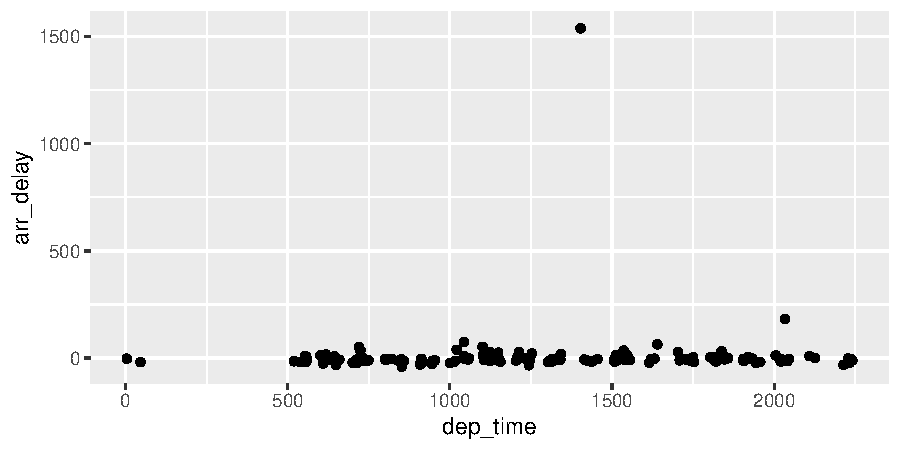
\includegraphics{Marc-Macarulay_files/figure-latex/march3plot-1.pdf}

\section{Additional resources}\label{additional-resources}
\begin{itemize}
\item
  \emph{Markdown} Cheatsheet -
  \url{https://github.com/adam-p/markdown-here/wiki/Markdown-Cheatsheet}
\item
  \emph{R Markdown} Reference Guide -
  \url{https://www.rstudio.com/wp-content/uploads/2015/03/rmarkdown-reference.pdf}
\item
  Introduction to \texttt{dplyr} -
  \url{https://cran.rstudio.com/web/packages/dplyr/vignettes/introduction.html}
\item
  \texttt{ggplot2} Documentation -
  \url{http://docs.ggplot2.org/current/}
\end{itemize}
\chapter{Methods}\label{math-sci}

\section{Study Setting and Study
Design}\label{study-setting-and-study-design}

The current study is an analysis of data compile

\hypertarget{ref-labels}{\chapter{Tables, Graphics, References, and
Labels}\label{ref-labels}}

\hypertarget{tables}{\section{Tables}\label{tables}}

By far the easiest way to present tables in your thesis is to store the
contents of the table in a CSV or Excel file, then read that file in to
your R Markdown document as a data frame. Then you can style the table
with the \texttt{kable} function, or functions in the
\href{https://cran.r-project.org/web/packages/kableExtra/index.html}{kableExtra}
pacakge.

In addition to the tables that can be automatically generated from a
data frame in \textbf{R} that you saw in {[}R Markdown Basics{]} using
the \texttt{kable} function, you can also create tables using
\emph{pandoc}. (More information is available at
\url{http://pandoc.org/README.html\#tables}.) This might be useful if
you don't have values specifically stored in \textbf{R}, but you'd like
to display them in table form. Below is an example. Pay careful
attention to the alignment in the table and hyphens to create the rows
and columns. Generally I don't recommend this approach of typing the
table directly into your R Markdown document.
\begin{longtable}[]{@{}ccc@{}}
\caption{\label{tab:inher} Correlation of Inheritance Factors for Parents
and Child}\tabularnewline
\toprule
\begin{minipage}[b]{0.29\columnwidth}\centering\strut
Factors\strut
\end{minipage} & \begin{minipage}[b]{0.47\columnwidth}\centering\strut
Correlation between Parents \& Child\strut
\end{minipage} & \begin{minipage}[b]{0.16\columnwidth}\centering\strut
Inherited\strut
\end{minipage}\tabularnewline
\midrule
\endfirsthead
\toprule
\begin{minipage}[b]{0.29\columnwidth}\centering\strut
Factors\strut
\end{minipage} & \begin{minipage}[b]{0.47\columnwidth}\centering\strut
Correlation between Parents \& Child\strut
\end{minipage} & \begin{minipage}[b]{0.16\columnwidth}\centering\strut
Inherited\strut
\end{minipage}\tabularnewline
\midrule
\endhead
\begin{minipage}[t]{0.29\columnwidth}\centering\strut
Education\strut
\end{minipage} & \begin{minipage}[t]{0.47\columnwidth}\centering\strut
-0.49\strut
\end{minipage} & \begin{minipage}[t]{0.16\columnwidth}\centering\strut
Yes\strut
\end{minipage}\tabularnewline
\begin{minipage}[t]{0.29\columnwidth}\centering\strut
Socio-Economic Status\strut
\end{minipage} & \begin{minipage}[t]{0.47\columnwidth}\centering\strut
0.28\strut
\end{minipage} & \begin{minipage}[t]{0.16\columnwidth}\centering\strut
Slight\strut
\end{minipage}\tabularnewline
\begin{minipage}[t]{0.29\columnwidth}\centering\strut
Income\strut
\end{minipage} & \begin{minipage}[t]{0.47\columnwidth}\centering\strut
0.08\strut
\end{minipage} & \begin{minipage}[t]{0.16\columnwidth}\centering\strut
No\strut
\end{minipage}\tabularnewline
\begin{minipage}[t]{0.29\columnwidth}\centering\strut
Family Size\strut
\end{minipage} & \begin{minipage}[t]{0.47\columnwidth}\centering\strut
0.18\strut
\end{minipage} & \begin{minipage}[t]{0.16\columnwidth}\centering\strut
Slight\strut
\end{minipage}\tabularnewline
\begin{minipage}[t]{0.29\columnwidth}\centering\strut
Occupational Prestige\strut
\end{minipage} & \begin{minipage}[t]{0.47\columnwidth}\centering\strut
0.21\strut
\end{minipage} & \begin{minipage}[t]{0.16\columnwidth}\centering\strut
Slight\strut
\end{minipage}\tabularnewline
\bottomrule
\end{longtable}
We can also create a link to the table by doing the following: Table
\ref{tab:inher}. If you go back to
\protect\hyperlink{loading-and-exploring-data}{Loading and exploring
data} and look at the \texttt{kable} table, we can create a reference to
this max delays table too: Table \ref{tab:maxdelays}. The addition of
the \texttt{(\textbackslash{}\#tab:inher)} option to the end of the
table caption allows us to then make a reference to Table
\texttt{\textbackslash{}@ref(tab:label)}. Note that this reference could
appear anywhere throughout the document after the table has appeared.

\clearpage

\section{Figures}\label{figures}

If your thesis has a lot of figures, \emph{R Markdown} might behave
better for you than that other word processor. One perk is that it will
automatically number the figures accordingly in each chapter. You'll
also be able to create a label for each figure, add a caption, and then
reference the figure in a way similar to what we saw with tables
earlier. If you label your figures, you can move the figures around and
\emph{R Markdown} will automatically adjust the numbering for you. No
need for you to remember! So that you don't have to get too far into
LaTeX to do this, a couple \textbf{R} functions have been created for
you to assist. You'll see their use below.

In the \textbf{R} chunk below, we will load in a picture stored as
\texttt{uw.png} in our main directory. We then give it the caption of
``UW logo'', the label of ``uwlogo'', and specify that this is a figure.
Make note of the different \textbf{R} chunk options that are given in
the R Markdown file (not shown in the knitted document).
\begin{Shaded}
\begin{Highlighting}[]
\KeywordTok{include_graphics}\NormalTok{(}\DataTypeTok{path =} \StringTok{"figure/uw.png"}\NormalTok{)}
\end{Highlighting}
\end{Shaded}
\begin{figure}
\centering

\includegraphics{figure/uw.png}
\caption{\label{fig:uwlogo}UW logo}
\end{figure}
Here is a reference to the UW logo: Figure \ref{fig:uwlogo}. Note the
use of the \texttt{fig:} code here. By naming the \textbf{R} chunk that
contains the figure, we can then reference that figure later as done in
the first sentence here. We can also specify the caption for the figure
via the R chunk option \texttt{fig.cap}.

\clearpage 

Below we will investigate how to save the output of an \textbf{R} plot
and label it in a way similar to that done above. Recall the
\texttt{flights} dataset from Chapter \ref{rmd-basics}. (Note that we've
shown a different way to reference a section or chapter here.) We will
next explore a bar graph with the mean flight departure delays by
airline from Portland for 2014. Note also the use of the \texttt{scale}
parameter which is discussed on the next page.
\begin{Shaded}
\begin{Highlighting}[]
\NormalTok{flights }\OperatorTok\StringTok{ }\KeywordTok{group_by}\NormalTok{(carrier) }\OperatorTok
\StringTok{  }\KeywordTok{summarize}\NormalTok{(}\DataTypeTok{mean_dep_delay =} \KeywordTok{mean}\NormalTok{(dep_delay)) }\OperatorTok
\StringTok{  }\KeywordTok{ggplot}\NormalTok{(}\KeywordTok{aes}\NormalTok{(}\DataTypeTok{x =}\NormalTok{ carrier, }\DataTypeTok{y =}\NormalTok{ mean_dep_delay)) }\OperatorTok{+}
\StringTok{  }\KeywordTok{geom_bar}\NormalTok{(}\DataTypeTok{position =} \StringTok{"identity"}\NormalTok{, }\DataTypeTok{stat =} \StringTok{"identity"}\NormalTok{, }\DataTypeTok{fill =} \StringTok{"red"}\NormalTok{)}
\end{Highlighting}
\end{Shaded}
\begin{figure}
\centering
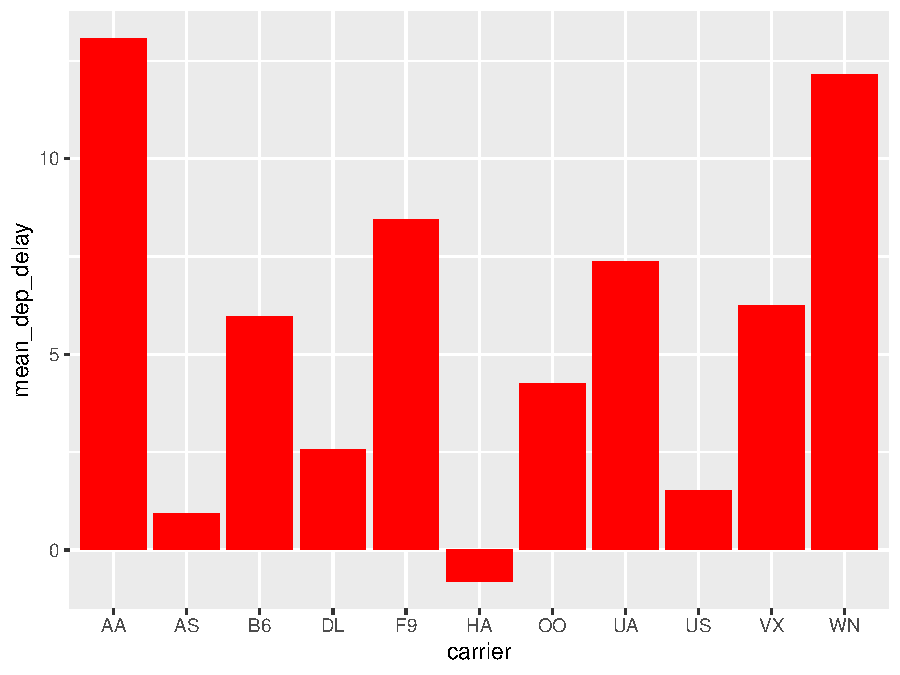
\includegraphics{Marc-Macarulay_files/figure-latex/delaysboxplot-1.pdf}
\caption{\label{fig:delaysboxplot}Mean Delays by Airline}
\end{figure}
Here is a reference to this image: Figure \ref{fig:delaysboxplot}.

A table linking these carrier codes to airline names is available at
\url{https://github.com/ismayc/pnwflights14/blob/master/data/airlines.csv}.

\clearpage

Next, we will explore the use of the \texttt{out.extra} chunk option,
which can be used to shrink or expand an image loaded from a file by
specifying \texttt{"scale=\ "}. Here we use the mathematical graph
stored in the ``subdivision.pdf'' file.
\begin{figure}
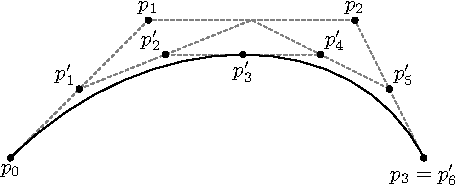
\includegraphics[scale=0.75]{figure/subdivision} \caption{Subdiv. graph}\label{fig:subd}
\end{figure}
Here is a reference to this image: Figure \ref{fig:subd}. Note that
\texttt{echo=FALSE} is specified so that the \textbf{R} code is hidden
in the document.

\textbf{More Figure Stuff}

Lastly, we will explore how to rotate and enlarge figures using the
\texttt{out.extra} chunk option. (Currently this only works in the PDF
version of the book.)
\begin{figure}
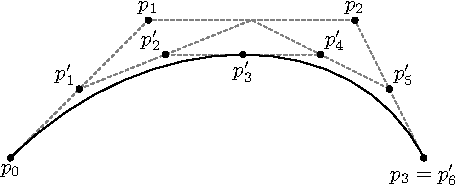
\includegraphics[angle=180, scale=1.1]{figure/subdivision} \caption{A Larger Figure, Flipped Upside Down}\label{fig:subd2}
\end{figure}
As another example, here is a reference: Figure \ref{fig:subd2}.

\section{Footnotes and Endnotes}\label{footnotes-and-endnotes}

You might want to footnote something.\footnote{footnote text} The
footnote will be in a smaller font and placed appropriately. Endnotes
work in much the same way.

\section{Cross-referencing chapters and
sections}\label{cross-referencing-chapters-and-sections}

The
\href{https://bookdown.org/yihui/bookdown/cross-references.html}{bookdown
documentation} is an excellent source for learning how to
cross-reference in a bookdown project such as a huskydown document. Here
we only cover the most common uses for a typical thesis. If you want
something more complex or fancy, please refer to the bookdown
documentation and seek help from the developers of that package.

By default, all of your chapter and section headers will get an
auto-generated ID label For example, e.g., \texttt{\#\ Chapter\ 1} will
have an auto-generated ID \texttt{chapter-1}. Note that the ID label is
all lower case, and has no spaces. If you have any kind of punctuation
in your header, such as a colon (:), it will not appear in the ID label.
Then in your text you can reference chapter one in your Rmd file like
this: `as discussed in Chapter
\texttt{\textbackslash{}@ref(chapter-1)}', which will print as `as
discussed in Chapter 1'

We strongly recommend that you to manually assign ID labels to your
chapter header to make it easy to cross-reference. For example, at the
top of the Rmd file for this chapter, you can see:

\texttt{\#\ Tables,\ Graphics,\ References,\ and\ Labels\ \{\#ref-labels\}}

The \texttt{\{\#ref-labels\}} part of this header is the ID label. It
doesn't show in the output, but is there for us to use for easy
cross-referencing, because it can be short, and we don't need to change
it elsewhere our document when we update the chapter header. We can use
this custom ID label in our Rmd document like this: `as discussed in
Chapter \texttt{\textbackslash{}@ref(ref-labels)}', which will print as
`as discussed in Chapter \ref{ref-labels}'. If you need to show custom
text instead of the chapter number, you use this syntax in your Rmd
document:
\texttt{see\ {[}my\ chapter\ about\ labels{]}(\#ref-labels)\ for\ more\ details}
which will appear as `see \protect\hyperlink{ref-labels}{my chapter
about labels} for more details'

To cross-reference a specific section in the same chapter, we recommend
adding a custom ID label to the section header, and using that to
cross-reference. For example, earlier in this chapter we have a section
on tables and in the Rmd file we see
\texttt{\#\#\ Tables\ \{\#tables\}}. We can cross-reference that in the
text like this `as discussed in the section on
\texttt{{[}tables{]}(\#tables)}' which will appear as `as discussed in
the above section on \protect\hyperlink{tables}{tables}'

To cross-reference a section in a different chapter we can use the ID
label from that section directly. For example, we can write in our Rmd
document
\texttt{as\ discussed\ in\ the\ section\ on\ {[}R\ code\ chunks{]}(\#r-chunks)\ in\ Chapter\ \textbackslash{}@ref(rmd-basics)}
which will appear as `as discussed in the section on
\protect\hyperlink{r-chunks}{R code chunks} in Chapter
\ref{rmd-basics}'.

If you prefer to cross-reference by the section number, we can use
custom ID labels in our Rmd document. For example, to refer to a section
in our first chapter, we can write in the Rmd document:
\texttt{as\ discussed\ in\ section\ \textbackslash{}@ref(r-chunks)\ in\ Chapter\ \textbackslash{}@ref(rmd-basics)}.
This will appear with section and chapter numbers like so: as `as
discussed in section \ref{r-chunks} in Chapter \ref{rmd-basics}'.

\section{Bibliographies}\label{bibliographies}

Of course you will need to cite things, and you will probably accumulate
an armful of sources. There are a variety of tools available for
creating a bibliography database (stored with the .bib extension). In
addition to BibTeX suggested below, you may want to consider using the
free and easy-to-use tool called Zotero. Some Zotero documentation is at
\url{http://libguides.reed.edu/citation/zotero}. In addition, a tutorial
is available from Middlebury College at
\url{http://sites.middlebury.edu/zoteromiddlebury/}.

\emph{R Markdown} uses \emph{pandoc} (\url{http://pandoc.org/}) to build
its bibliographies. One nice caveat of this is that you won't have to do
a second compile to load in references as standard LaTeX requires. To
cite references in your thesis (after creating your bibliography
database), place the reference name inside square brackets and precede
it by the ``at'' symbol. For example, here's a reference to a book about
worrying: ({\textbf{???}}). This \texttt{Molina1994} entry appears in a
file called \texttt{thesis.bib} in the \texttt{bib} folder. This
bibliography database file was created by a program called BibTeX. You
can call this file something else if you like (look at the YAML header
in the main .Rmd file) and, by default, is to placed in the \texttt{bib}
folder.

For more information about BibTeX and bibliographies, see
(\url{http://web.reed.edu/cis/help/latex/index.html})\footnote{({\textbf{???}})}.
There are three pages on this topic: \emph{bibtex} (which talks about
using BibTeX, at \url{http://web.reed.edu/cis/help/latex/bibtex.html}),
\emph{bibtexstyles} (about how to find and use the bibliography style
that best suits your needs, at
\url{http://web.reed.edu/cis/help/latex/bibtexstyles.html}) and
\emph{bibman} (which covers how to make and maintain a bibliography by
hand, without BibTeX, at
\url{http://web.reed.edu/cis/help/latex/bibman.html}). The last page
will not be useful unless you have only a few sources.

If you look at the YAML header at the top of the main .Rmd file you can
see that we can specify the style of the bibliography by referencing the
appropriate csl file. You can download a variety of different style
files at \url{https://www.zotero.org/styles}. Make sure to download the
file into the csl folder.

\textbf{Tips for Bibliographies}
\begin{itemize}
\tightlist
\item
  Like with thesis formatting, the sooner you start compiling your
  bibliography for something as large as thesis, the better.
\item
  The cite key (a citation's label) needs to be unique from the other
  entries.
\item
  When you have more than one author or editor, you need to separate
  each author's name by the word ``and'' e.g.
  \texttt{Author\ =\ \{Noble,\ Sam\ and\ Youngberg,\ Jessica\},}.
\item
  Bibliographies made using BibTeX (whether manually or using a manager)
  accept LaTeX markup, so you can italicize and add symbols as
  necessary.
\item
  To force capitalization in an article title or where all lowercase is
  generally used, bracket the capital letter in curly braces.
\end{itemize}
\section{Anything else?}\label{anything-else}

If you'd like to see examples of other things in this template, please
\href{https://github.com/benmarwick/huskydown/issues/new}{contact us}
(email \href{mailto:bmarwick@uw.edu}{\nolinkurl{bmarwick@uw.edu}}) with
your suggestions. We love to see people using \emph{R Markdown} for
their theses, and are happy to help.

\chapter*{Conclusion}\label{conclusion}
\addcontentsline{toc}{chapter}{Conclusion}

If we don't want Conclusion to have a chapter number next to it, we can
add the \texttt{\{-\}} attribute.

\textbf{More info}

And here's some other random info: the first paragraph after a chapter
title or section head \emph{shouldn't be} indented, because indents are
to tell the reader that you're starting a new paragraph. Since that's
obvious after a chapter or section title, proper typesetting doesn't add
an indent there.

\appendix

\chapter{The First Appendix}\label{the-first-appendix}

This first appendix includes all of the R chunks of code that were
hidden throughout the document (using the \texttt{include\ =\ FALSE}
chunk tag) to help with readibility and/or setup.

\textbf{In the main Rmd file}
\begin{Shaded}
\begin{Highlighting}[]
\CommentTok{# This chunk ensures that the huskydown package is}
\CommentTok{# installed and loaded. This huskydown package includes}
\CommentTok{# the template files for the thesis.}
\ControlFlowTok{if}\NormalTok{(}\OperatorTok{!}\KeywordTok{require}\NormalTok{(devtools))}
  \KeywordTok{install.packages}\NormalTok{(}\StringTok{"devtools"}\NormalTok{, }\DataTypeTok{repos =} \StringTok{"http://cran.rstudio.com"}\NormalTok{)}
\ControlFlowTok{if}\NormalTok{(}\OperatorTok{!}\KeywordTok{require}\NormalTok{(huskydown))}
\NormalTok{  devtools}\OperatorTok{::}\KeywordTok{install_github}\NormalTok{(}\StringTok{"benmarwick/huskydown"}\NormalTok{)}
\KeywordTok{library}\NormalTok{(huskydown)}
\end{Highlighting}
\end{Shaded}
\textbf{In Chapter \ref{ref-labels}:}
\begin{Shaded}
\begin{Highlighting}[]
\CommentTok{# This chunk ensures that the huskydown package is}
\CommentTok{# installed and loaded. This huskydown package includes}
\CommentTok{# the template files for the thesis and also two functions}
\CommentTok{# used for labeling and referencing}
\ControlFlowTok{if}\NormalTok{(}\OperatorTok{!}\KeywordTok{require}\NormalTok{(devtools))}
  \KeywordTok{install.packages}\NormalTok{(}\StringTok{"devtools"}\NormalTok{, }\DataTypeTok{repos =} \StringTok{"http://cran.rstudio.com"}\NormalTok{)}
\ControlFlowTok{if}\NormalTok{(}\OperatorTok{!}\KeywordTok{require}\NormalTok{(dplyr))}
    \KeywordTok{install.packages}\NormalTok{(}\StringTok{"dplyr"}\NormalTok{, }\DataTypeTok{repos =} \StringTok{"http://cran.rstudio.com"}\NormalTok{)}
\ControlFlowTok{if}\NormalTok{(}\OperatorTok{!}\KeywordTok{require}\NormalTok{(ggplot2))}
    \KeywordTok{install.packages}\NormalTok{(}\StringTok{"ggplot2"}\NormalTok{, }\DataTypeTok{repos =} \StringTok{"http://cran.rstudio.com"}\NormalTok{)}
\ControlFlowTok{if}\NormalTok{(}\OperatorTok{!}\KeywordTok{require}\NormalTok{(ggplot2))}
    \KeywordTok{install.packages}\NormalTok{(}\StringTok{"bookdown"}\NormalTok{, }\DataTypeTok{repos =} \StringTok{"http://cran.rstudio.com"}\NormalTok{)}
\ControlFlowTok{if}\NormalTok{(}\OperatorTok{!}\KeywordTok{require}\NormalTok{(huskydown))\{}
  \KeywordTok{library}\NormalTok{(devtools)}
\NormalTok{  devtools}\OperatorTok{::}\KeywordTok{install_github}\NormalTok{(}\StringTok{"benmarwick/huskydown"}\NormalTok{)}
\NormalTok{  \}}
\KeywordTok{library}\NormalTok{(huskydown)}
\NormalTok{flights <-}\StringTok{ }\KeywordTok{read.csv}\NormalTok{(}\StringTok{"data/flights.csv"}\NormalTok{)}
\end{Highlighting}
\end{Shaded}
\chapter{The Second Appendix, for
Fun}\label{the-second-appendix-for-fun}

\chapter*{Colophon}\label{colophon}
\addcontentsline{toc}{chapter}{Colophon}

This document is set in \href{https://github.com/georgd/EB-Garamond}{EB
Garamond}, \href{https://github.com/adobe-fonts/source-code-pro/}{Source
Code Pro} and \href{http://www.latofonts.com/lato-free-fonts/}{Lato}.
The body text is set at 11pt with \(\familydefault\).

It was written in R Markdown and \(\LaTeX\), and rendered into PDF using
\href{https://github.com/benmarwick/huskydown}{huskydown} and
\href{https://github.com/rstudio/bookdown}{bookdown}.

This document was typeset using the XeTeX typesetting system, and the
\href{http://staff.washington.edu/fox/tex/}{University of Washington
Thesis class} class created by Jim Fox. Under the hood, the
\href{https://github.com/UWIT-IAM/UWThesis}{University of Washington
Thesis LaTeX template} is used to ensure that documents conform
precisely to submission standards. Other elements of the document
formatting source code have been taken from the
\href{https://github.com/stevenpollack/ucbthesis}{Latex, Knitr, and
RMarkdown templates for UC Berkeley's graduate thesis}, and
\href{https://github.com/suchow/Dissertate}{Dissertate: a LaTeX
dissertation template to support the production and typesetting of a PhD
dissertation at Harvard, Princeton, and NYU}

The source files for this thesis, along with all the data files, have
been organised into an R package, xxx, which is available at
\url{https://github.com/xxx/xxx}. A hard copy of the thesis can be found
in the University of Washington library.

This version of the thesis was generated on 2020-05-11 14:44:11. The
repository is currently at this commit:

The computational environment that was used to generate this version is
as follows:
\begin{verbatim}
- Session info ---------------------------------------------------------------
 setting  value                       
 version  R version 3.6.1 (2019-07-05)
 os       Windows 10 x64              
 system   x86_64, mingw32             
 ui       RTerm                       
 language (EN)                        
 collate  English_United States.1252  
 ctype    English_United States.1252  
 tz       America/Los_Angeles         
 date     2020-05-11                  

- Packages -------------------------------------------------------------------
 package     * version date       lib source                               
 assertthat    0.2.1   2019-03-21 [1] CRAN (R 3.6.1)                       
 backports     1.1.4   2019-04-10 [1] CRAN (R 3.6.0)                       
 bookdown      0.18.1  2020-05-01 [1] Github (rstudio/bookdown@cd97d40)    
 callr         3.3.1   2019-07-18 [1] CRAN (R 3.6.1)                       
 cli           1.1.0   2019-03-19 [1] CRAN (R 3.6.1)                       
 colorspace    1.4-1   2019-03-18 [1] CRAN (R 3.6.1)                       
 crayon        1.3.4   2017-09-16 [1] CRAN (R 3.6.1)                       
 desc          1.2.0   2018-05-01 [1] CRAN (R 3.6.2)                       
 devtools    * 2.2.1   2019-09-24 [1] CRAN (R 3.6.2)                       
 digest        0.6.20  2019-07-04 [1] CRAN (R 3.6.1)                       
 dplyr       * 0.8.3   2019-07-04 [1] CRAN (R 3.6.1)                       
 ellipsis      0.3.0   2019-09-20 [1] CRAN (R 3.6.2)                       
 evaluate      0.14    2019-05-28 [1] CRAN (R 3.6.1)                       
 fs            1.3.1   2019-05-06 [1] CRAN (R 3.6.1)                       
 ggplot2     * 3.2.0   2019-06-16 [1] CRAN (R 3.6.0)                       
 git2r         0.26.1  2019-06-29 [1] CRAN (R 3.6.2)                       
 glue          1.3.1   2019-03-12 [1] CRAN (R 3.6.1)                       
 gtable        0.3.0   2019-03-25 [1] CRAN (R 3.6.1)                       
 highr         0.8     2019-03-20 [1] CRAN (R 3.6.1)                       
 htmltools     0.4.0   2019-10-04 [1] CRAN (R 3.6.2)                       
 huskydown   * 0.0.5   2020-05-01 [1] Github (benmarwick/huskydown@a909835)
 knitr       * 1.27    2020-01-16 [1] CRAN (R 3.6.2)                       
 labeling      0.3     2014-08-23 [1] CRAN (R 3.6.0)                       
 lazyeval      0.2.2   2019-03-15 [1] CRAN (R 3.6.1)                       
 magrittr      1.5     2014-11-22 [1] CRAN (R 3.6.1)                       
 memoise       1.1.0   2017-04-21 [1] CRAN (R 3.6.2)                       
 munsell       0.5.0   2018-06-12 [1] CRAN (R 3.6.1)                       
 pillar        1.4.2   2019-06-29 [1] CRAN (R 3.6.1)                       
 pkgbuild      1.0.6   2019-10-09 [1] CRAN (R 3.6.2)                       
 pkgconfig     2.0.2   2018-08-16 [1] CRAN (R 3.6.1)                       
 pkgload       1.0.2   2018-10-29 [1] CRAN (R 3.6.2)                       
 prettyunits   1.0.2   2015-07-13 [1] CRAN (R 3.6.1)                       
 processx      3.4.0   2019-07-03 [1] CRAN (R 3.6.1)                       
 ps            1.3.0   2018-12-21 [1] CRAN (R 3.6.1)                       
 purrr         0.3.3   2019-10-18 [1] CRAN (R 3.6.2)                       
 R6            2.4.0   2019-02-14 [1] CRAN (R 3.6.1)                       
 Rcpp          1.0.1   2019-03-17 [1] CRAN (R 3.6.1)                       
 remotes       2.1.0   2019-06-24 [1] CRAN (R 3.6.2)                       
 rlang         0.4.3   2020-01-24 [1] CRAN (R 3.6.2)                       
 rmarkdown     2.1     2020-01-20 [1] CRAN (R 3.6.3)                       
 rprojroot     1.3-2   2018-01-03 [1] CRAN (R 3.6.1)                       
 rstudioapi    0.10    2019-03-19 [1] CRAN (R 3.6.1)                       
 scales        1.0.0   2018-08-09 [1] CRAN (R 3.6.1)                       
 sessioninfo   1.1.1   2018-11-05 [1] CRAN (R 3.6.2)                       
 stringi       1.4.3   2019-03-12 [1] CRAN (R 3.6.0)                       
 stringr       1.4.0   2019-02-10 [1] CRAN (R 3.6.1)                       
 testthat      2.3.1   2019-12-01 [1] CRAN (R 3.6.2)                       
 tibble        2.1.3   2019-06-06 [1] CRAN (R 3.6.1)                       
 tidyselect    0.2.5   2018-10-11 [1] CRAN (R 3.6.1)                       
 usethis     * 1.6.1   2020-04-29 [1] CRAN (R 3.6.3)                       
 withr         2.1.2   2018-03-15 [1] CRAN (R 3.6.1)                       
 xfun          0.8     2019-06-25 [1] CRAN (R 3.6.1)                       
 yaml          2.2.0   2018-07-25 [1] CRAN (R 3.6.0)                       

[1] C:/Users/Marc/Documents/R/win-library/3.6
[2] C:/Program Files/R/R-3.6.1/library
\end{verbatim}
\backmatter

\chapter*{References}\label{references}
\addcontentsline{toc}{chapter}{References}

\markboth{References}{References}

\noindent

\setlength{\parindent}{-0.20in} \setlength{\leftskip}{0.20in}
\setlength{\parskip}{8pt}

\hypertarget{refs}{}
\hypertarget{ref-Keene2018}{}
Keene, D. E., Guo, M., \& Murillo, S. (2018). ``That wasn't really a
place to worry about diabetes'': Housing access and diabetes
self-management among low-income adults. \emph{Social Science \&
Medicine}, \emph{197}, 71--77.
\url{http://doi.org/10.1016/J.SOCSCIMED.2017.11.051}
\end{document}
